%
% File coling2020.tex
%
% Contact: feiliu@cs.ucf.edu & liang.huang.sh@gmail.com
%% Based on the style files for COLING-2018, which were, in turn,
%% Based on the style files for COLING-2016, which were, in turn,
%% Based on the style files for COLING-2014, which were, in turn,
%% Based on the style files for ACL-2014, which were, in turn,
%% Based on the style files for ACL-2013, which were, in turn,
%% Based on the style files for ACL-2012, which were, in turn,
%% based on the style files for ACL-2011, which were, in turn, 
%% based on the style files for ACL-2010, which were, in turn, 
%% based on the style files for ACL-IJCNLP-2009, which were, in turn,
%% based on the style files for EACL-2009 and IJCNLP-2008...

%% Based on the style files for EACL 2006 by 
%%e.agirre@ehu.es or Sergi.Balari@uab.es
%% and that of ACL 08 by Joakim Nivre and Noah Smith

\documentclass[11pt]{article}
\usepackage{coling2020}
\usepackage{times}
\usepackage{url}
\usepackage{latexsym}
\usepackage{indentfirst}

\usepackage{times}
\usepackage{latexsym}
\usepackage{times}
\usepackage{soul}
\usepackage{url}
\usepackage{amsmath}
\usepackage{amsthm}
\usepackage{booktabs}
\usepackage{algorithm}
\usepackage{algorithmic}
\usepackage{amssymb}
\usepackage{longtable}
\usepackage{graphicx}
\usepackage{CJK}
\usepackage{multirow}
\usepackage{color}

%\setlength\titlebox{5cm}
\colingfinalcopy % Uncomment this line for the final submission

% You can expand the titlebox if you need extra space
% to show all the authors. Please do not make the titlebox
% smaller than 5cm (the original size); we will check this
% in the camera-ready version and ask you to change it back.


\title{2021年03月07日进度汇报}

\author{屈原斌 \\
  首都师范大学 \\
    {\tt ybqu@cnu.edu.cn}}

\date{}

\begin{document}
\begin{CJK}{UTF8}{gkai}

\maketitle
\CJKindent
%\begin{abstract}

%\end{abstract}

\section{今日进度}


\begin{itemize}
\item [1.] 整理英文实验结果
\item [2.] 跑Bert生成实验
\item [3.] 英文生成模型可视化
\item [4.] 准备reading group PPT
\end{itemize}

\section{结论}
\begin{itemize}
  \item 英文seq2seq生成模型指标,见Table 1
  \item 离题实验指标更新,见Table2、Table 3:
  \item 方案:
  \begin{itemize}
    \item 方案一:基于题目排序方法,见图1
    \begin{figure*}[htbp]\small
      \centering
      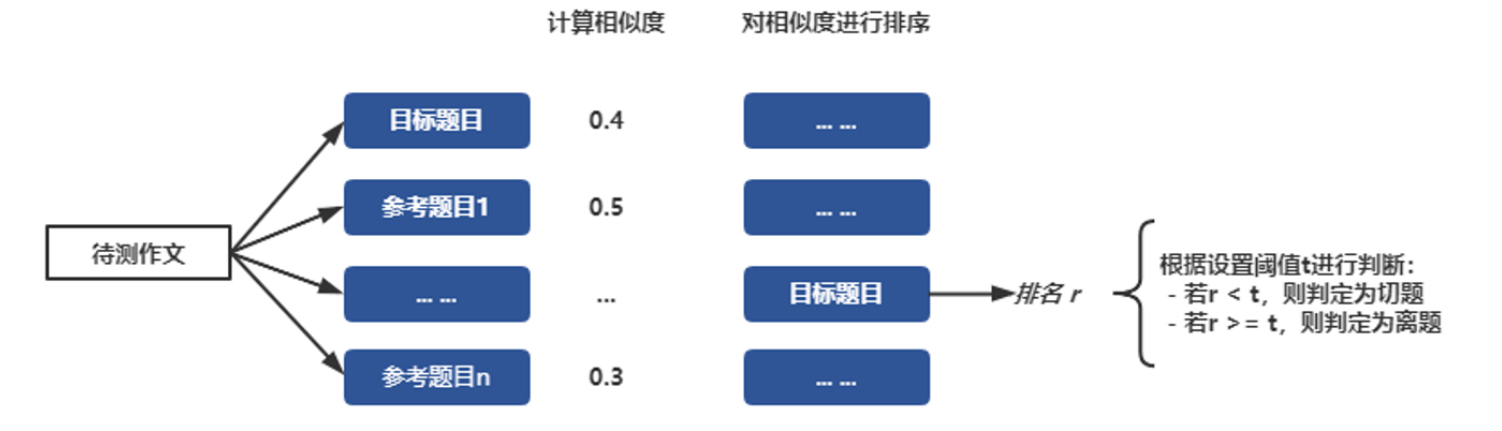
\includegraphics[width=1.0\linewidth]{fa1.png}
      \caption{基于题目排序方法}
      \label{framework}
    \end{figure*}
    \item 方案二:基于相似度方法,见图2
    \begin{figure*}[htbp]\small
      \centering
      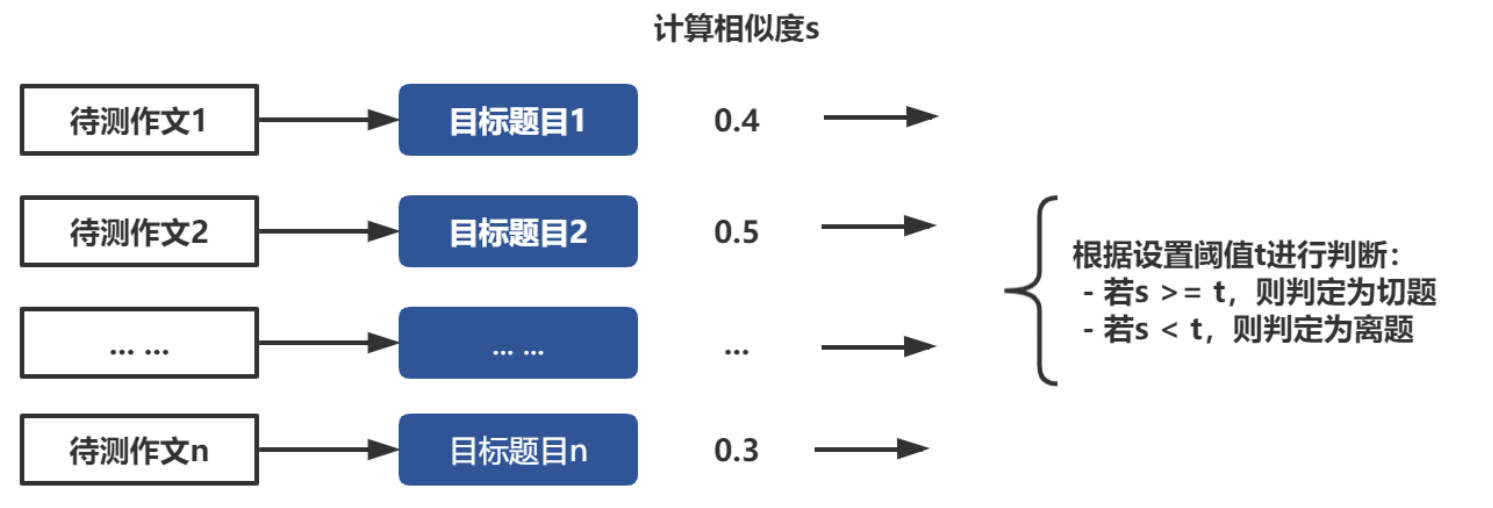
\includegraphics[width=1.0\linewidth]{fa2.png}
      \caption{基于相似度方法}
      \label{framework}
    \end{figure*}
  \end{itemize}
  \item 结论:
  \begin{itemize}
    \item 方案一指标优于方案二
    \item 使用F1调阈值时不离题指标下降
  \end{itemize}
\end{itemize}



% Table generated by Excel2LaTeX from sheet 'Sheet2'
\begin{table}[htbp]
  \centering
  \begin{tabular}{c|c|c}
    \hline
    \multicolumn{2}{c|}{} & \textbf{rouge\_l} \\
    \hline
    \multirow{2}[0]{*}{\textbf{BiLstm}} & \textbf{MLE} & \multicolumn{1}{c}{0.3150 } \\
    \cline{2-3}
    & \textbf{+RL} & 0.3212  \\
    \hline
  \end{tabular}%
  \caption{生成模型指标}
  \label{tab:addlabel}%
\end{table}%

% Table generated by Excel2LaTeX from sheet 'Sheet3'
% Table generated by Excel2LaTeX from sheet 'Sheet3'
\begin{table}[htbp]
  \centering
  \begin{tabular}{cc|c|ccc|ccc}
    \hline
    \multicolumn{2}{c}{\multirow{2}[0]{*}{}} & \multirow{2}[0]{*}{Accuracy} & \multicolumn{3}{c}{\textbf{离题}} & \multicolumn{3}{c}{\textbf{不离题}} \\
    \multicolumn{2}{c}{} &       & \textbf{precision} & \textbf{recall} & \textbf{f1-score} & \textbf{precision} & \textbf{recall} & \textbf{f1-score} \\
    \hline
    \multirow{2}[0]{*}{\textbf{离题F1-score}} & \textbf{开发集} & \textbf{-} & 0.4779  & 0.9544  & 0.6361  & 0.6811  & 0.0893  & 0.1558  \\
    & \textbf{测试集} & \textbf{-} & 0.4724  & 0.9463  & \textcolor{red}{0.6301}  & 0.6293  & 0.0766  & 0.1352  \\
    \hline
    \multirow{2}[0]{*}{\textbf{Accuracy}} & \textbf{开发集} & \textbf{0.5831 } & 0.5769  & 0.5028  & 0.5206  & 0.6025  & 0.6540  & 0.6163  \\
    & \textbf{测试集} & \textbf{0.5416 } & 0.5100  & 0.4617  & 0.4715  & 0.5684  & 0.6100  & 0.5792  \\
    \hline
  \end{tabular}%
  \caption{方案一指标更新}
  \label{tab:addlabel}%
\end{table}%

% Table generated by Excel2LaTeX from sheet 'Sheet3'
\begin{table}[htbp]
  \centering
  \begin{tabular}{cc|c|ccc|ccc}
    \hline
    \multicolumn{2}{c}{\multirow{2}[0]{*}{}} & \multirow{2}[0]{*}{Accuracy} & \multicolumn{3}{c}{\textbf{离题}} & \multicolumn{3}{c}{\textbf{不离题}} \\
    \multicolumn{2}{c}{} &       & \textbf{precision} & \textbf{recall} & \textbf{f1-score} & \textbf{precision} & \textbf{recall} & \textbf{f1-score} \\
    \hline
    \multirow{2}[0]{*}{\textbf{离题F1-score}} & \textbf{开发集} & \textbf{-} & 0.5861  & 0.1208  & 0.1815  & 0.5537  & 0.9471  & 0.6964  \\
    & \textbf{测试集} & \textbf{-} & 0.3033  & 0.0908  & 0.1355  & 0.5368  & 0.9196  & 0.6766  \\
    \hline
    \multirow{2}[0]{*}{\textbf{Accuracy}} & \textbf{开发集} & \textbf{0.5602 } & 0.5861  & 0.1208  & 0.1815  & 0.5537  & 0.9471  & 0.6964  \\
    & \textbf{测试集} & \textbf{0.5334 } & 0.3033  & 0.0908  & 0.1355  & 0.5368  & 0.9196  & 0.6766  \\
    \hline
  \end{tabular}%
  \caption{方案二指标更新}
  \label{tab:addlabel}%
\end{table}%





% Table generated by Excel2LaTeX from sheet '中文数据集'
% \begin{figure*}[htbp]\small
%   \centering
%   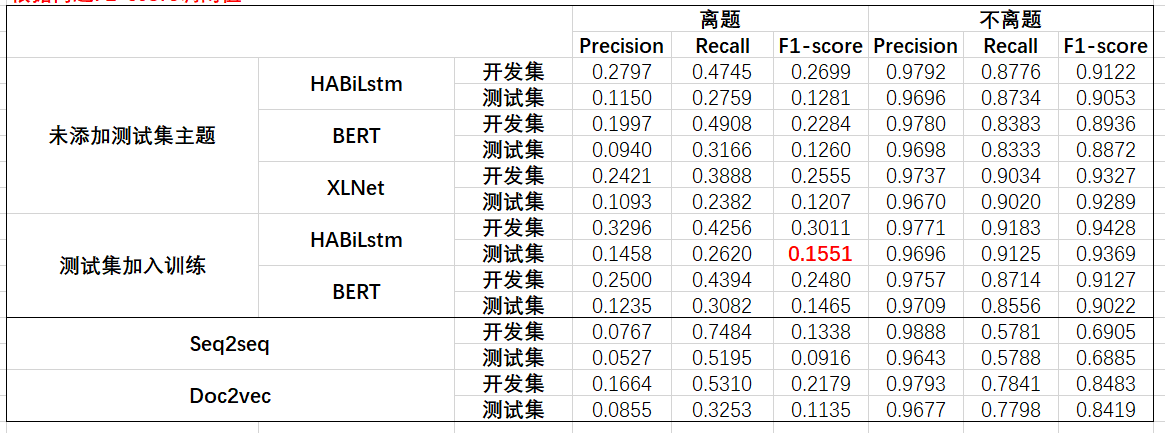
\includegraphics[width=1.0\linewidth]{zb.png}
%   \caption{生成样例2}
%   \label{framework}
% \end{figure*}

%\bibliography{reference}
%\bibliographystyle{coling}
%\bibliography{coling2020}

\end{CJK}
\end{document}


% include your own bib file like this:


%\begin{thebibliography}{}

%\bibitem[\protect\citename{Aho and Ullman}1972]{Aho:72}
%Alfred~V. Aho and Jeffrey~D. Ullman.
%\newblock 1972.
%\newblock {\em The Theory of Parsing, Translation and Compiling}, volume~1.
%\newblock Prentice-{Hall}, Englewood Cliffs, NJ.

%\bibitem[\protect\citename{{American Psychological Association}}1983]{APA:83}
%{American Psychological Association}.
%\newblock 1983.
%\newblock {\em Publications Manual}.
%\newblock American Psychological Association, Washington, DC.

%\bibitem[\protect\citename{{Association for Computing Machinery}}1983]{ACM:83}
%{Association for Computing Machinery}.
%\newblock 1983.
%\newblock {\em Computing Reviews}, 24(11):503--512.

%\bibitem[\protect\citename{Chandra \bgroup et al.\egroup }1981]{Chandra:81}
%Ashok~K. Chandra, Dexter~C. Kozen, and Larry~J. Stockmeyer.
%\newblock 1981.
%\newblock Alternation.
%\newblock {\em Journal of the Association for Computing Machinery},
%  28(1):114--133.

%\bibitem[\protect\citename{Gusfield}1997]{Gusfield:97}
%Dan Gusfield.
%\newblock 1997.
%\newblock {\em Algorithms on Strings, Trees and Sequences}.
%\newblock Cambridge University Press, Cambridge, UK.

%\bibitem[\protect\citename{Rasooli and Tetreault}2015]{rasooli-tetrault-2015}
%Mohammad~Sadegh Rasooli and Joel~R. Tetreault. 2015.
%\newblock {Yara parser: {A} fast and accurate dependency parser}.
%\newblock \emph{Computing Research Repository}, arXiv:1503.06733.
%\newblock Version 2.

%\bibitem[\protect\citename{Borschinger and Johnson}2011]{borsch2011}
%Benjamin Borschinger and Mark Johnson. 2011.
%\newblock A particle filter algorithm for {B}ayesian wordsegmentation.
%\newblock In \emph{Proceedings of the Australasian Language Technology Association %Workshop 2011}, pages 10--18, Canberra, Australia.

%\end{thebibliography}

